%% Begin slides template file
\documentclass[11pt,t,usepdftitle=false,aspectratio=169]{beamer}
%% ------------------------------------------------------------------
%% - aspectratio=43: Set paper aspect ratio to 4:3.
%% - aspectratio=169: Set paper aspect ratio to 16:9.
%% ------------------------------------------------------------------
\usepackage{graphicx}
\usetheme[nototalframenumber,logo,license]{uibk}
%% ------------------------------------------------------------------
%% - foot: Add a footer line for conference name and date.
%% - logo: Add the university logo in the footer (only if 'foot' set).
%% - bigfoot/sasquatch: Larger font size in footer.
%% - nototalslidenumber: Hide the total number of slides (only if 'foot' set)
%% - license: Add CC-BY license symbol to title slide (e.g., for conference uploads)
%%   (TODO: At the moment no other licenses are supported.)
%% - licenseall: Add CC-BY license symbol to all subsequent slides slides
%% - url: use \url{} rather than \href{} on the title page
%% ------------------------------------------------------------------

%% ------------------------------------------------------------------
%% The official corporate colors of the university are predefined and
%% can be used for e.g., highlighting something. Simply use
%% \color{uibkorange} or \begin{color}{uibkorange} ... \end{color}
%% Defined colors are:
%% - uibkblue, uibkbluel, uibkorange, uibkorangel, uibkgray, uibkgraym, uibkgrayl
%% The frametitle color can be easily adjusted e.g., to black with
%% \setbeamercolor{titlelike}{fg=black}
%% ------------------------------------------------------------------

%\setbeamercolor{verbcolor}{fg=uibkorange}
%% ------------------------------------------------------------------
%% Setting a highlight color for verbatim output such as from
%% the commands \pkg, \email, \file, \dataset
%% ------------------------------------------------------------------


%% information for the title page ('short title' is the pdf-title that is shown in viewer's titlebar)
\title[IoT Light Bulb Attack]{IoT Light Bulb Covert Channel}
\subtitle{Extended Functionality Attack on Smart Lights}
\URL{}

\author[Julia Wanker \& Bennett Piater]{Julia Wanker, Bennett Piater}
%('short author' is the pdf-metadata Author)
%% If multiple authors are required and the font size is too large you
%% can overrule the font size of author and url by calling:
%\setbeamerfont{author}{size*={10pt}{10pt},series=\mdseries}
%\setbeamerfont{url}{size*={10pt}{10pt},series=\mdseries}
%\URL{}
%\subtitle{}

\footertext{}
\date{2017-07-25}

\headerimage{3}
%% ------------------------------------------------------------------
%% The theme offers four different header images based on the
%% corporate design of the university of innsbruck. Currently
%% 1, 2, 3 and 4 is allowed as input to \headerimage{...}. Default
%% or fallback is '1'.
%% ------------------------------------------------------------------

\begin{document}

%% ALTERNATIVE TITLEPAGE
%% The next block is how you add a titlepage with the 'nosectiontitlepage' option, which switches off
%% the default behavior of creating a titlepage every time a \section{} is defined.
%% Then you can use \section{} as it's originally intended, including a table of contents.
% \usebackgroundtemplate{\includegraphics[width=\paperwidth,height=\paperheight]{titlebackground.pdf}}
% \begin{frame}[plain]
%     \titlepage
% \end{frame}
% \addtocounter{framenumber}{-1}
% \usebackgroundtemplate{}}

%% Table of Contents, if wanted:
%% this requires the 'nosectiontitlepage' option and setting \section{}'s as you want them to appear here.
%% Subsections and subordinates are suppressed in the .sty at the moment, search
%% for \setbeamertemplate{subsection} and replace the empty {} with whatever you want.
%% Although it's probably too much for a presentation, maybe for a lecture.
% \begin{frame}
%     \vspace*{1cm plus 1fil}
%     \tableofcontents
%     \vspace*{0cm plus 1fil}
% \end{frame}

%%%%%%%%%%%%%%%%%%%%%%%%%%%%%%%%%%%%%%%%%%%%%%%%%%%%%%%%%%%%%%%%%%%%%%%%%
% Intro:
% - names
% - topic
% - structure: First Taxonomy (main paper), then overview of main paper and possible related work
%%%%%%%%%%%%%%%%%%%%%%%%%%%%%%%%%%%%%%%%%%%%%%%%%%%%%%%%%%%%%%%%%%%%%%%%%

%% this sets the first PDF bookmark and triggers generation of the title page
\section{Taxonomy of IoT Attacks}
\begin{frame}{Taxonomy of IoT Attacks}
	\begin{enumerate}
		\item Ignoring Functionality
		\item Reducing Functionality
		\item Misusing Functionality
		\item Extending Functionality
	\end{enumerate}
	\note{Briefly introduce the taxonomy to give viewers an overview.}
\end{frame}

%% this just generates PDF bookmarks
\subsection{Ignoring Functionality}
\begin{frame}{Ignoring Functionality}
	% TODO talk about about DDoS, Mirai? Probably a graph of DDoS growth or something.

	% The low security and network-attachment of IoT devices makes them perfect for botnets.
	% And their low computing power makes them comparatively highly suitable for DDoS attacks (or spam).

	% presentation-wise, definitely some visualization.
	\pause{}
	\begin{figure}
		\centering
		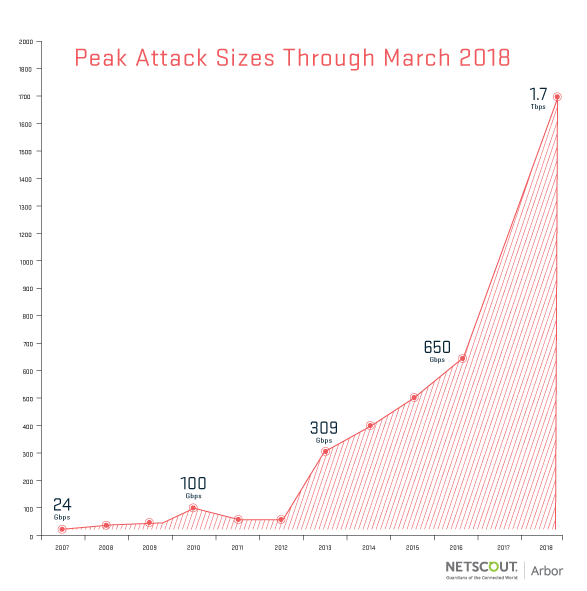
\includegraphics[keepaspectratio,height=.85 \paperheight]{img/DDoS_growth}
	\end{figure}
\end{frame}

\subsection{Reducing Functionality}
\begin{frame}{Reducing Functionality}
	% TODO Find examples of this in practice.
	% We probably can cite something about disabling lights from one of our papers.
	% Other nice things would be fridges or tvs, maybe we can find that?
	% This can dangerous: a smart fridge that thaws meat every night can be deadly!
	% https://www.infoworld.com/article/3176673/internet-of-things/your-smart-fridge-may-kill-you-the-dark-side-of-iot.html

	% presentation-wise, probably just bullet-points?
\end{frame}

\subsection{Misusing Functionality}
\begin{frame}{Misusing Functionality}
	\begin{block}{Create Discomfort}
		\begin{itemize}
			\item Heat in summer, AC in winter
			\item Flash bedroom lights at night
			\item Turn on AC in bathroom in the morning
		\end{itemize}
	\end{block}
	\begin{block}{Generally be Annoying}
		\begin{itemize}
			\item Turn on lights
			\item Open Faucets
			\item Run Washing Machine
		\end{itemize}
		\dots~when the owners leave for vacation.
	\end{block}
\end{frame}

\subsection{Extending Functionality}
	% TODO The interesting things. I like the examples from the paper:
	% Start a fire with AC, unlock front door with roomba (vacuum cleaner robot)

	% Any idea of how to visualize that?
\begin{frame}{Extending Functionality}

\end{frame}

\title{Ronen, Shamir Paper}
\subtitle{}
\section{Ronen, Shamir Paper}

\subsection{Covert Channel}%
\label{sub:covert_channel}

\subsubsection{Requirements for Covert Channel}%
\label{sub:requirements_for_covert_channel}
\begin{frame}{Requirements for Covert Channel}
	\begin{block}{Correctness}
		Switch between 2 brightnesses that can be robustly distinguished by a sensor.
	\end{block}
	\begin{block}{Covertness}
		Use brightnesses so similar or switch so fast that a human cannot distinguish them.
	\end{block}
\end{frame}
% with info about human eyes

\subsubsection{How (smart) LEDs work}%
\label{sub:how_smart_leds_work}
% TODO
% with info about controller, ZLL, and PWM duty cycle for brightness
% Probably want to add a duty cycle/brightness diagram or something.

\subsubsection{Encoding: Crafting of PWM Signals}%
\label{sub:encoding_crafting_of_pwm_signals}
% TODO
% - Talk about attacking/using the controller
% - Talk about how to make sufficiently fast changes
% - Diagram of the resulting signals?

% Need to think about whether we want to cover LimitlessLED/LUX old/LUX new or only one of them!

\subsubsection{Decoding: Light Sensor Signal Analysis}%
\label{sub:decoding_light_sensor_signal_analysis}
% TODO
% - Describe receiving hardware setup
% - Describe how the signal can be processed to get a bit stream

\subsubsection{Why this Paper is Important for this Topic}%
\label{sub:why_this_paper_is_important_for_this_topic}
% TODO
% Because it's the only one covering this topic, quite simply^^


\subsection{Epilepsy Triggering Attack}%
\label{sub:epilepsy_triggering_attack}
% TODO Either we only mention it, or we expand it into a full .5 minutes slide.
% Depends on whether we need to fill time I guess.

%% to show a last slide similar to the title slide: information for the last page
\title{Questions?}
\subtitle{}
\section{Questions}


%% appendix of 'extra' slides
\appendix

\end{document}

% vim: spell ts=2 sw=2
